\documentclass[a4paper, french]{article}
\usepackage{config}
\author{Vincent Commin \& Louis Leenart}
\date{\today}
\setcounter{secnumdepth}{6}
\begin{document}

\begin{titlepage}
    \begin{flushleft}
        
\includegraphics[width=5cm]{UL.jpg}\par
        \centering

        \vspace{13\baselineskip}
        \HRule \\[0.4cm]

        {\Huge
        GIF-4104 - TP 4\par}
        \vspace{0.4cm}
        \HRule
        \vfill
        Équipe 1 : Vincent Commin \& Louis Leenart\medskip \par
    \end{flushleft}
\end{titlepage}

\newpage
\section{Introduction}

Pour ce quatrième TP, nous avons implémenté la parallélisation d'inversion d'une matrice en utilisant
méthode de \href{https://fr.wikipedia.org/wiki/%C3%89limination_de_Gauss-Jordan}{\textit{\underline{Gauss Jordan}}}
avec  \href{https://www.khronos.org/opencl/}{\textit{\underline{OpenCL}}} et \href{https://www.openacc.org/}{\textit{\underline{OpenACC}}}. En se basant sur l'implémentation séquentielle proposée, nous avons suivi l'approche par réduction puis diffusion successives.

\section{Notre approche}

\subsection{OpenCL}

Dans ce TP, nous avons découvert l'utilisation d'OpenCL ainsi que ses particularités. En implémentant l'algorithme d'inversion de matrix de Gauss Jordan pour une architecture de GPU, nous avions en tête de diminuer le temps de calcul pour qu'il soit inférieur à celui obtenu avec l'utilisation uniquement du CPU.

L'algorithme que nous avons mis en place est le suivant :

\begin{lstlisting}[style=txt]
AI : Matrix [A I] // Shared amoung every GPU threads
Buffer : value array // Shared amoung every GPU
size, rank : integer

FOR k = 0 TO AI.rows DO
    max = 0, pivotIndex = k
    FOR i = k TO AI.rows DO // Find greatest pivot for column k
        IF (i mod size) == rank && abs(AI[i, k]) > max DO
            max = abs(AI[i, k]); pivotIndex = i
        DONE
    DONE

    Buffer[pivotIndex] = max
    pivotIndex = Reduce(MAX_LOG, Buffer) // Location of max value in Buffer

    IF IA[pivotIndex, k] == 0 DO throw exception DONE

    v = AI[k, k] // Normalisation
    FOR j = 0 TO AI.cols DO
        AI[k, j] = AI[k, j] / v
    DONE

    FOR i = 0 TO AI.rows DO // For each rows
        IF i mod size == rank && i != k DO
            AI[i] -= AI[k] * AI[i, k]
        DONE
    DONE
DONE

FOR i = 0 TO AI.rows DO // Copy right side of AI into result
    A = AI.getData()[slice(i * AI.cols + AI.rows, AI.rows, 1)]
DONE
\end{lstlisting}

L'utilisation que nous avons fait d'OpenCL est assez naïve : découvrant le langage, nous avons simplement essayé d'appliquer l'algorithme d'inversion. Pas encore suffisament familier avec les tenants et aboutissants de chacun des paramètres OpenCL, nous avons eu du mal à paramétrer ce dernier pour maximiser les performances. Nous avons par ailleurs remarqué que pour une taille de workgroup plus grande que 128, des erreurs de calculs ont commencé à appaitre, mais nous avons pas réussi à identifier la source de ce problème, c'est pourquoi nous conduirons nos calculs pour des matrix de taille maximum 128 x 128.

D'après les spécifications de la carte graphique utilisée, nous avons décidé d'utiliser un worker group de la taille de la matrice, et donc d'associer une ligne à chacun des worker, ce qui nous a permi d'obtenir les meilleurs résultats. La minimisation de l'accès à la mémoire globale n'a pu être notre priorité, et l'on remarque effectivement que chaque worker accède régulièrement à la mémoire globale ce qui n'est pas obtimal.

\subsection{OpenACC}

Pour la version utilisant OpenACC, nous avons décidé de reprendre le programme séquentiel et d'y ajouter les directives comme il ait conseillé. Nous avons, comme pour le programme OpenCL, décidé de paralléliser la fonction d'inversion de matrice par la méthode de Gauss-Jordan.

L'algorithme que nous avons mis en place est le suivant :

\begin{lstlisting}[style=txt]
AI : Matrix [A I]

// local matrix initialize as identity matrix
// concatenated with the AI matrix
lAI : Identity Matrix [A I]

// Give lAI and AI matrix as input and output
// for every inner parallel sections
#pragma acc data copy(lAI, AI)
{
FOR k = 0 TO AI.rows DO
    max = abs(lAI[i, k]), pivotIndex = k
    FOR i = k TO lAI.rows DO // Find greatest pivot for column k
        IF abs(lAI[i, k]) > max DO
            max = abs(lAI[i, k]); pivotIndex = i
        DONE
    DONE

    IF lIA[pivotIndex, k] == 0 DO throw exception DONE
    IF (pivotIndex != k) AI.swapRows(pivotIndex, k)

    v = lAI[k, k] // Normalisation
    // Parrallelize the for loop passing lValue and k as output only
    #pragma acc parallel loop copyin(lValue, k)
    FOR j = 0 TO lAI.cols DO
        lAI[k, j] = lAI[k, j] / v
    DONE

    // Parrallelize the for loop, as k is already present in
    // the device memory, we reuse it
    #pragma acc parallel loop present(k)
    FOR i = 0 TO lAI.rows DO // For each rows
        IF i != k DO
            lAI[i] = lAI[i] - lAI[k] * v
        DONE
    DONE
DONE

#pragma acc parallel loop
FOR i = 0 TO AI.rows DO // Copy right side of AI into result
    AI[i] = lAI.getData()[slice(i * lAI.cols + AI.cols, AI.cols, 1)]
DONE
}
\end{lstlisting}

L'avantage de OpenACC est de pouvoir réutiliser le code séquentiel afin de la paralléliser. De plus, ce que OpenACC parrallélise le plus facilement sont les boucles, c'est pour cela que toutes les directives se trouvent aux abords de celles-ci. Avant d'utiliser les directives de parallélisation, nous faisons appel à la directive \textbf{data} qui nous permet de passer les matrices \textbf{lAI} et \textbf{AI} en lecture et écriture à toutes les autres directives de parallélisation inclues dans cette directive \textbf{data}.

Pour la première boucle récupérant l'index du maximum, il aurait été intéressant d'utilisant la clause de réduction sur la fonction \textbf{max}. Cependant, cela est rendu impossible par l'assignation de l'index. Nous avons donc fait le choix de ne pas paralléliser cette boucle, cela aurait été du calcul redondant sur tout les threads ce qui aurait diminué l'efficacité.

\section{Machine utilisée pour les tests de performance}

\begin{center}
    \begin{tabularx}{0.6\textwidth}{|>{\raggedleft\arraybackslash}X|>{\raggedright\arraybackslash}X|}
        \hline
        Modèle & intel i7-8550U \\
        \hline
        Architecture & x86\_64 \\
        \hline
        OS & Archlinux \\
        \hline
        Fréquence CPU & 3.4GHz \\
        \hline
        C\oe urs (physique / logique) & 4 / 8 \\
        \hline
        Ram & 16 Go, 2400 $MT/s$ \\
        \hline
        GPU & Intel(R) UHD Graphics 620 \\
        \hline
        OpenCL & version 3.0 \\
        \hline
        GCC & version 11.2.0 \\
        \hline
        nvc++ & version 22.1 \\
        \hline
    \end{tabularx}
\end{center}

\section{Résultats obtenus}

\begin{center}
    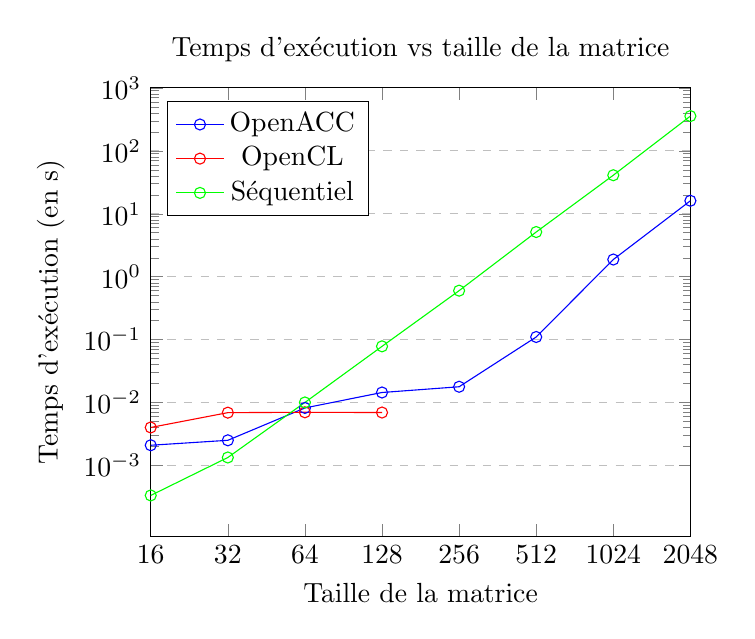
\begin{tikzpicture}
        \begin{axis}[
            xmode=log,
            ymode=log,
            log basis x={2},
            title={Temps d'exécution vs taille de la matrice},
            xlabel={Taille de la matrice},
            ylabel={Temps d'exécution (en s)},
            xmin=16, xmax=2048,
            ymin=0, ymax=1000,
            xtick={16,32,64,128, 256, 512, 1024, 2048},
            ytick={0,0.001, 0.01, 0.1, 1, 10, 100, 1000},
            legend pos=north west,
            ymajorgrids=true,
            grid style=dashed,
            xticklabels={16,32,64,128, 256, 512, 1024, 2048}
            ]
            \addplot[color=blue, mark=o] coordinates {(16, 0.00210473)(32,0.00252273)(64,0.0082381)(128,0.0144982)(256,0.0178835)(512,0.110395)(1024,1.8773)(2048,16.0946)};
            \addplot[color=red, mark=o] coordinates {(16, 0.004035)(32, 0.006936)(64, 0.007028)(128, 0.006966)};
            \addplot[color=green, mark=o] coordinates {(16, 0.000335783)(32,0.00134538)(64,0.0100722)(128,0.0784007)(256,0.601008)(512,5.13331)(1024,40.9636)(2048,356.321)};
            \legend{OpenACC, OpenCL, Séquentiel}
        \end{axis}
    \end{tikzpicture}
\end{center}

\newpage

\section{Analyse}

Tout d'abord, nous avons conduit l'étude selon les conditions suivantes : le temps séquentiel correspond à l'utilisation de l'algorithme en compilant sans OpenACC (avec nvc++), donc en utilisant un seul fil d'execution CPU. Concernant OpenACC, notre GPU (intel) n'est pas compatible avec la compilation via nvc++, il n'a été possible que de compiler en utilisant le paramètre multicore, ciblant uniquement le CPU. À noter que nous avons eu de grandes difficultés à tenter de compiler notre programme avec GCC, cependant lui non plus ne supporte pas les GPU intel. Enfin, OpenCL utilise évidemment le GPU intel, cependant nous avons remarqué que l'algorithme rencontre de nombreuses erreurs quand la matrice devient trop grande (à partir de 128 environ) d'où l'absence de données.

On note l'absence des valeurs de speedup et d'efficacité, en effet, l'efficacité dépend du nombre de processus utilisés par rapport au temps séquentiel, hors ici pour OpenCL on compare le temps séquentiel au temps GPU (les processus fonctionnent différemment, cela n'a pas de sens de comparer), et pour OpenACC, nous utilisons un autre compilateur (NVC++) qui semble donner des performances significativement différentes.

D'après les résultats obtenus, on remarque que le temps de calcul pour OpenACC est significativement plus faible que le temps séquentiel (échelle logarithmique), même si le taux de croissance est identique. En effet, comme nous utilisons le même algorithme ayant une complexité de $O(n^3)$. On peut constater que le temps de calcul pour OpenCL est du même ordre qu'OpenACC, cependant, la limite de taille de matrice calculé rend difficile l'analyse de la tendance. Comme cet algorithme est le seul que nous avons
pu executer sur notre GPU en utilisant le parrallélisme, nous pourrions nous attendre à une
variation du temps de calcul en fonction de la taille de la matrice significativement différente par rappport aux cas d’utilisation du CPU.

Vu que nos algorithmes sont exécutés dans un contexte relativement différent (utilisation du CPU et du GPU), comparer les performances est complexe. Cependant, une analyse naïve du temps de calcul par rapport à la taille de la matrice nous permet de remarquer que l'utilisation d'OpenACC et NVC++ permet un temps de calcul significativement inférieur par rapport au calcul séquentiel avec GCC. Aussi, l'utilisation d'OpenCL dans des conditions non obtimales (code peu optimisé) semble aussi performant, voire même plus performant qu'OpenACC.

\section{Conclusion}

Lors de ce TP, nous avons rencontré plusieurs difficultés. Dans un premier temps, pour la mise en place d'un système de compilation performant et compatible (notamment pour OpenACC), nous sommes passés par l'utilisation de NVC++, puis par la recompilation de GCC (avec les bons modules pour espérer compiler pour GPU intel), puis de nouveau par NVC++ étant donné l'absence de support des compilateurs pour notre hardware. Concernant OpenCL, novices au langage, nous avons eu des difficultés à obtenir un algorithme fonctionnel, cependant ce dernier rencontre encore aujourd'hui des limitations. Nous avons aussi essayé de profiler notre GPU pour obtenir plus d'informations quant aux performances, sans succès.

Nous avons  pu étudier la programmation sur GPU, et obtenir des résultats de performance intéressants.
Lors de nos recherches pour mieux comprendre l'algorithme de Gauss Jordan, nous avons trouvé le travail de \href{https://dro.deakin.edu.au/view/DU:30044550}{\textit{\underline{Lau, K. K., Kumar, M. J. et Venkatesh, S., Parallel matrix inversion techniques}}}\footnote{https://dro.deakin.edu.au/view/DU:30044550} proposant une variation cet algorithme, notamment pour les systèmes SIMD, atteignant une complexité temporelle de $O(n)$, avec n la taille de la matrice. Ils proposent aussi une implémentation pour les systèmes MIMD avec une complexité de $O(\frac{n}{m})$, avec n la taille de la matrice et m le nombre de machines dans le système. L'implémentant de ces variations mèneraient à des performances encore un peu plus avancées, tout en conservant la méthode d'élimination Gaussienne.

\end{document}